\chapter{Discussion}

\section{Interdisciplinary Interpretation}
The section is based on a discussion with Dr. Jessica (Yi Xuan) Luo, psychiatry registrar at Northern Hospital, Epping. We compared the results of our analysis with \cite[Fig. 1]{stern2011}. \cref{fig:interdis} collects the necessary information for this discussion.
\begin{figure}[H]
  \centering
  \begin{subfigure}[b]{0.32\textwidth}
    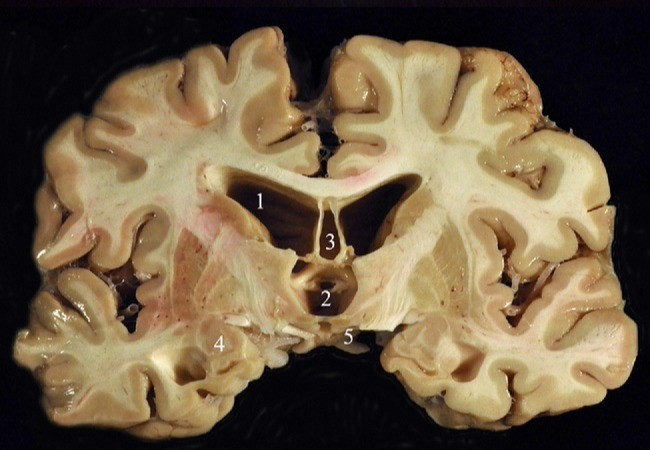
\includegraphics[width=\linewidth]{cte.jpg}
    \caption{CTE brain from \cite[Fig. 1]{stern2011}}\label{fig:i1}
  \end{subfigure}\hfill
  \begin{subfigure}[b]{0.32\textwidth}
    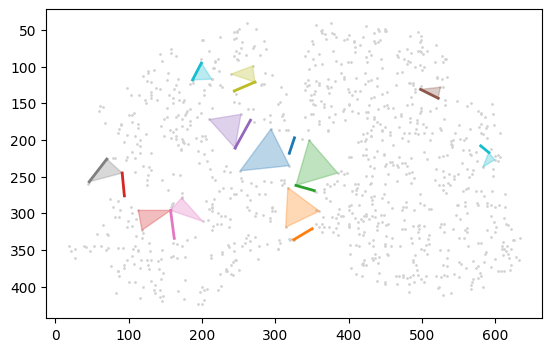
\includegraphics[width=\linewidth]{cte_features.png}
    \caption{CTE Point Cloud with Highlighted Features}\label{fig:i2}
  \end{subfigure}\hfill
  \begin{subfigure}[b]{0.32\textwidth}
    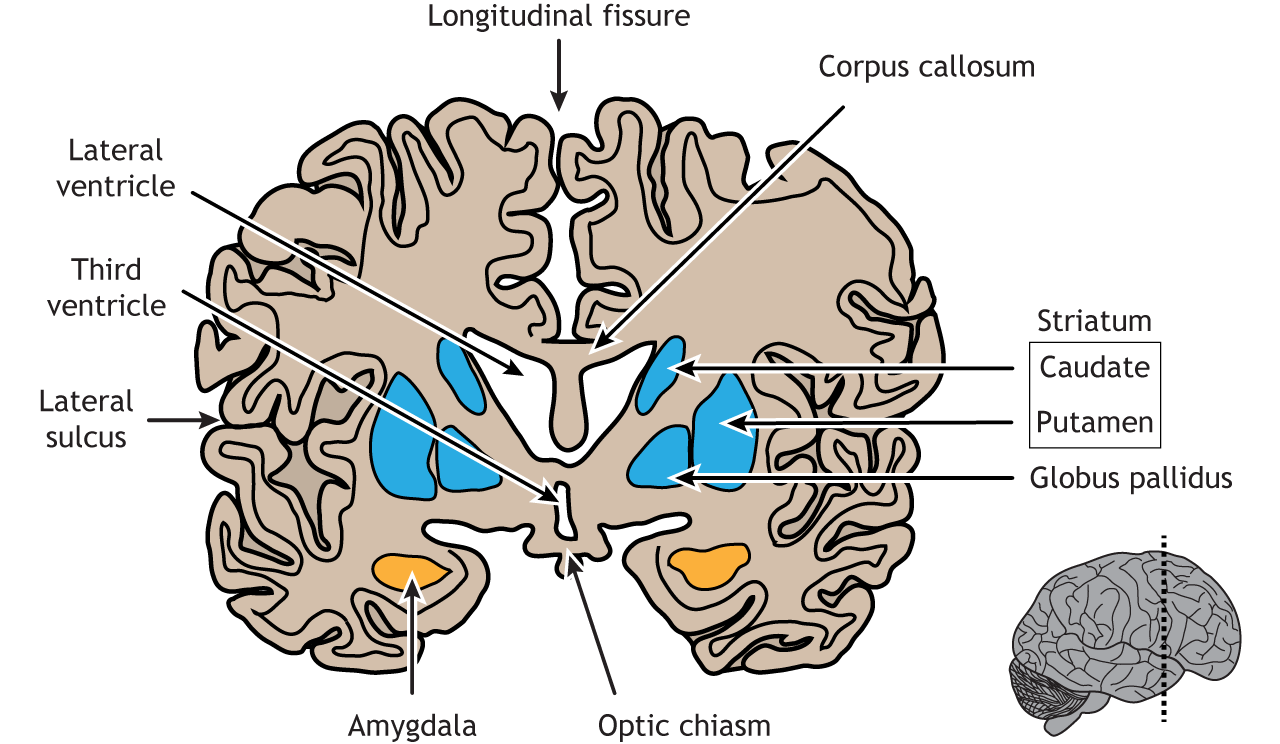
\includegraphics[width=\linewidth]{Coronal-Amygdala.png}
    \caption{Labelled coronal section of the brain \cite[Fig. 20.3]{henley_amygdala_bg} }\label{fig:i3}
  \end{subfigure}
  \caption{Overall caption for the panel.}\label{fig:interdis}
\end{figure}
\noindent
In \cref{fig:i1}, the authors identify five differences between the gross pathology of the control and CTE brain:
\begin{enumerate}
    \item Severe dilatation of ventricle II.
    \item Severe dilatation of ventricle III.
    \item Severe dilatation of cavum septum pellucidum.
    \item Marked atrophy of the medial temporal lobe structures.
    \item Shrinkage of the mammillary bodies.
\end{enumerate}
Items 1,2, and 3 are characteristic of overall brain shrinkage. The ventricles and cavum septum pellucidum are responsible for nourishing the brain with cerebrospinal fluid. When that process is inhibited, overall brain function breaks down. In \cref{fig:i2}, we observe features (blue, green, orange) that seem to coincide with Items 1, 2, and 3.
\\\\
Item 4 describes the death of the temporal lobe. This includes the hippocampus, responsible for memory, and the amygdala, responsible for emotional regulation. Thus, it is not surprising that as that region is impacted those with CTE suffer from memory and emotional dysfunction. Whilst we observe features (light pink, dark pink) in \cref{fig:i2} that are near this region, they seem to be focused on the dilatated lateral sulcus (see \cref{fig:i3}), which is a corollary of overall brain shrinkage rather than a cause for specific concern. Atrophy refers to overall shrinkage, rather than creation of holes or cavities, which is why TDA may not have detected it.
\\\\
Item 5 describes the shrinkage of the mammillary bodies, part of the limbic system, which manage many unconscious bodily instincts, like survival. Like Item 4, TDA does not detect this shrinkage.
\\\\
Several other features (black, brown, light blue) are identified in \cref{fig:i2}. However, each of them seem to be cavities created by overall brain shrinkage.
\\\\
In this instance, TDA provided no advantage over a clinician looking at the images. TDA could not detect some features and detected others that were spurious. 

\section{Limitations}\label{limitations}
Two practical factors influenced many decisions in this report: (i) we had one semester (12 weeks) to complete the analysis and report, and (ii) computation time and power was limited.
\\\\
Additionally, my learning goal for this report was to implement TDA in a practical setting. As such, some choices were made to maximise those goals, and in a professional setting other choices may have been better.
\\\\
In this chapter, we discuss various limitations of this report.
\begin{enumerate}
    \item Our study design compares only one CTE and one control brain. In part, this choice was made in the interests of time. 
    \\\\
    There are also ethical concerns: many deaths due to CTE occur amongst high-profile athletes, and often their brains are donated to science on the condition of anonymity. Thus, outside of research institutes like Boston University's CTE Center or the University of Sydney's Australian Sports Brain Bank, large datasets are not available.
    \\\\
    Hypothetically, a similar analysis conducted on a larger dataset should also incorporate other variables, such as sport played, number of concussions, concussion symptoms, etc, into its analysis. 
    \item In \cref{tda}, we introduced TDA as our main analytic tool for this report. TDA is not necessarily the best tool for this analysis, and there are several limitations worth discussing.
    \begin{itemize}
        \item TDA renders a fundamentally smooth object (in this case, a brain) as a discrete mathematical object (a point cloud). There is no guarantee that the point cloud is a faithful approximation of the original smooth object. Mathematically speaking, a manifold or Riemannian surface may be a sounder representation, and analytic techniques under this assumption may be profitable, for example in \cite{john2025shape}.
        \item A central tenant of TDA is the use of topological, or shape-based, information. However, it is extremely difficult to interpret results in dimension $\geq 4$. In this report, we simply ignored these higher dimensional features, which potentially ignores important information.
        \item TDA is inherently computationally expensive because the number of simplices formed from a point cloud grows exponentially. Thus, we really have only ourself to blame for many of the computational limitations.
        \item By definition, TDA detects differences in shape that alter topological invariants, like the number of holes. Features that do not alter topological invariants, for example the overall shrinkage of a part of the brain, may therefore be missed by TDA.
    \end{itemize}
    \item In \cref{preproc}, we removed the author annotations on the CTE brain with Adobe Express Online's wand tool. We made this choice in the interests of time, but it introduces exterior noise to the image. An ideal approach would have been to contact the original authors of the paper and ask for a high resolution copy of the image.
    \item \label{graylim} In \cref{proc}, we rendered the images in grayscale to simplify their conversion to a point cloud. Fundamentally, this ignores colour as a variable. An approach that may have mitigated this problem is \textit{persistent homology for multispecies data}, a technique developed in \cite{MR4798124}, by treating different coloured pixels as different species of data. 
    \item \label{brightlim} In \cref{proc}, we chose an arbitrary brightness threshold of $0.5$. An alternative route could have been to repeat the analysis for a variety of thresholds and interpret the results as a collective.
    \item In \cref{comparison}, we used a resampling procedure as a stand-in for parametric hypothesis testing. This could be improved by computing many resamples of the point clouds and reporting an empirical confidence interval from the collection of distances. We did not pursue this step due to the computational time required.
\end{enumerate}


\section{Reflection}
In this report, I sought to extend my knowledge in three ways:
\begin{enumerate}
    \item Topology is a field of mathematics that I am less familiar with. My Master's research was in algebraic combinatorics, so it was challenging to engage with a topic I did not have strong foundations in.
    \item My Master's research was almost entirely theoretical. Whilst we used computer programming (mainly Mathematica) to check examples and build intuition, we did not have to make computational decisions or interpretations. Those goals, as well as coding in Python, was new to me in this report.
    \item I chose an example from psychiatry in this report because it gave me an opportunity to engage in interdisciplinary research with my friend Dr. Jessica Luo. This process extended my professional and interpersonal skills, and improved the focus of the report.
\end{enumerate}
\noindent
The biggest challenge I faced in this report was bringing together the theoretical knowledge of TDA I had learnt with the practical considerations of being a beginner programmer with limited resources. Often, the theory told me what I \textit{should} do, but I was limited in what I \textit{could} do. 
\\\\
For example, I had learnt the theory of how to compare persistence diagrams but it was not clear how one should actually interpret the bottleneck or Wasserstein distance in practice. My solution was to resample the point clouds and use the Control vs Resample and CTE vs Resample distances as benchmarks for the Control vs CTE distances I was trying to understand.






 
